% Digital Logic Report Template
% Created: 2020-01-10, John Miller

%==========================================================
%=========== Document Setup  ==============================

% Formatting defined by class file
\documentclass[11pt]{article}

% ---- Document formatting ----
\usepackage[margin=1in]{geometry}	% Narrower margins
\usepackage{booktabs}				% Nice formatting of tables
\usepackage{graphicx}				% Ability to include graphics

%\setlength\parindent{0pt}	% Do not indent first line of paragraphs 
\usepackage[parfill]{parskip}		% Line space b/w paragraphs
%	parfill option prevents last line of pgrph from being fully justified

% Parskip package adds too much space around titles, fix with this
\RequirePackage{titlesec}
\titlespacing\section{0pt}{8pt plus 4pt minus 2pt}{3pt plus 2pt minus 2pt}
\titlespacing\subsection{0pt}{4pt plus 4pt minus 2pt}{-2pt plus 2pt minus 2pt}
\titlespacing\subsubsection{0pt}{2pt plus 4pt minus 2pt}{-6pt plus 2pt minus 2pt}

% ---- Hyperlinks ----
\usepackage[colorlinks=true,urlcolor=blue]{hyperref}	% For URL's. Automatically links internal references.

% ---- Code listings ----
\usepackage{listings} 					% Nice code layout and inclusion
\usepackage[usenames,dvipsnames]{xcolor}	% Colors (needs to be defined before using colors)

% Define custom colors for listings
\definecolor{listinggray}{gray}{0.98}		% Listings background color
\definecolor{rulegray}{gray}{0.7}			% Listings rule/frame color

% Style for Verilog
\lstdefinestyle{Verilog}{
	language=Verilog,					% Verilog
	backgroundcolor=\color{listinggray},	% light gray background
	rulecolor=\color{blue}, 			% blue frame lines
	frame=tb,							% lines above & below
	linewidth=\columnwidth, 			% set line width
	basicstyle=\small\ttfamily,	% basic font style that is used for the code	
	breaklines=true, 					% allow breaking across columns/pages
	tabsize=3,							% set tab size
	commentstyle=\color{gray},	% comments in italic 
	stringstyle=\upshape,				% strings are printed in normal font
	showspaces=false,					% don't underscore spaces
}

% How to use: \Verilog[listing_options]{file}
\newcommand{\Verilog}[2][]{%
	\lstinputlisting[style=Verilog,#1]{#2}
}




%======================================================
%=========== Body  ====================================
\begin{document}

\title{ELC 2137 Lab 1: Lab Title}
\author{Victoria Covey}

\maketitle


\section*{Summary}

In this experiment, I was able to learn how to use the version control software, GitHub, and use it to download/upload, save, and modify various files. Of these files, many of them used LaTeX, a typesetting language. After learning specifics about this language, I was able to download and work on a .tex file.


\section*{Q\&A}
\begin{enumerate}
	\item What is your GitHub user name?
	
	VictoriaCovey
	
	\item What LaTeX environment produces a bulleted (non-numbered) list?
	
	enumerate
	
	\item Write  the  \verb5equation y(t) = 1/2 e^t5 using  La-TeX equation formatting.
	
	$y(t)= \frac{1}{2}e^t$
	
	\item  What is the shortcut key for compiling your La-TeX document?
	
	F5
\end{enumerate}

\section*{Results}

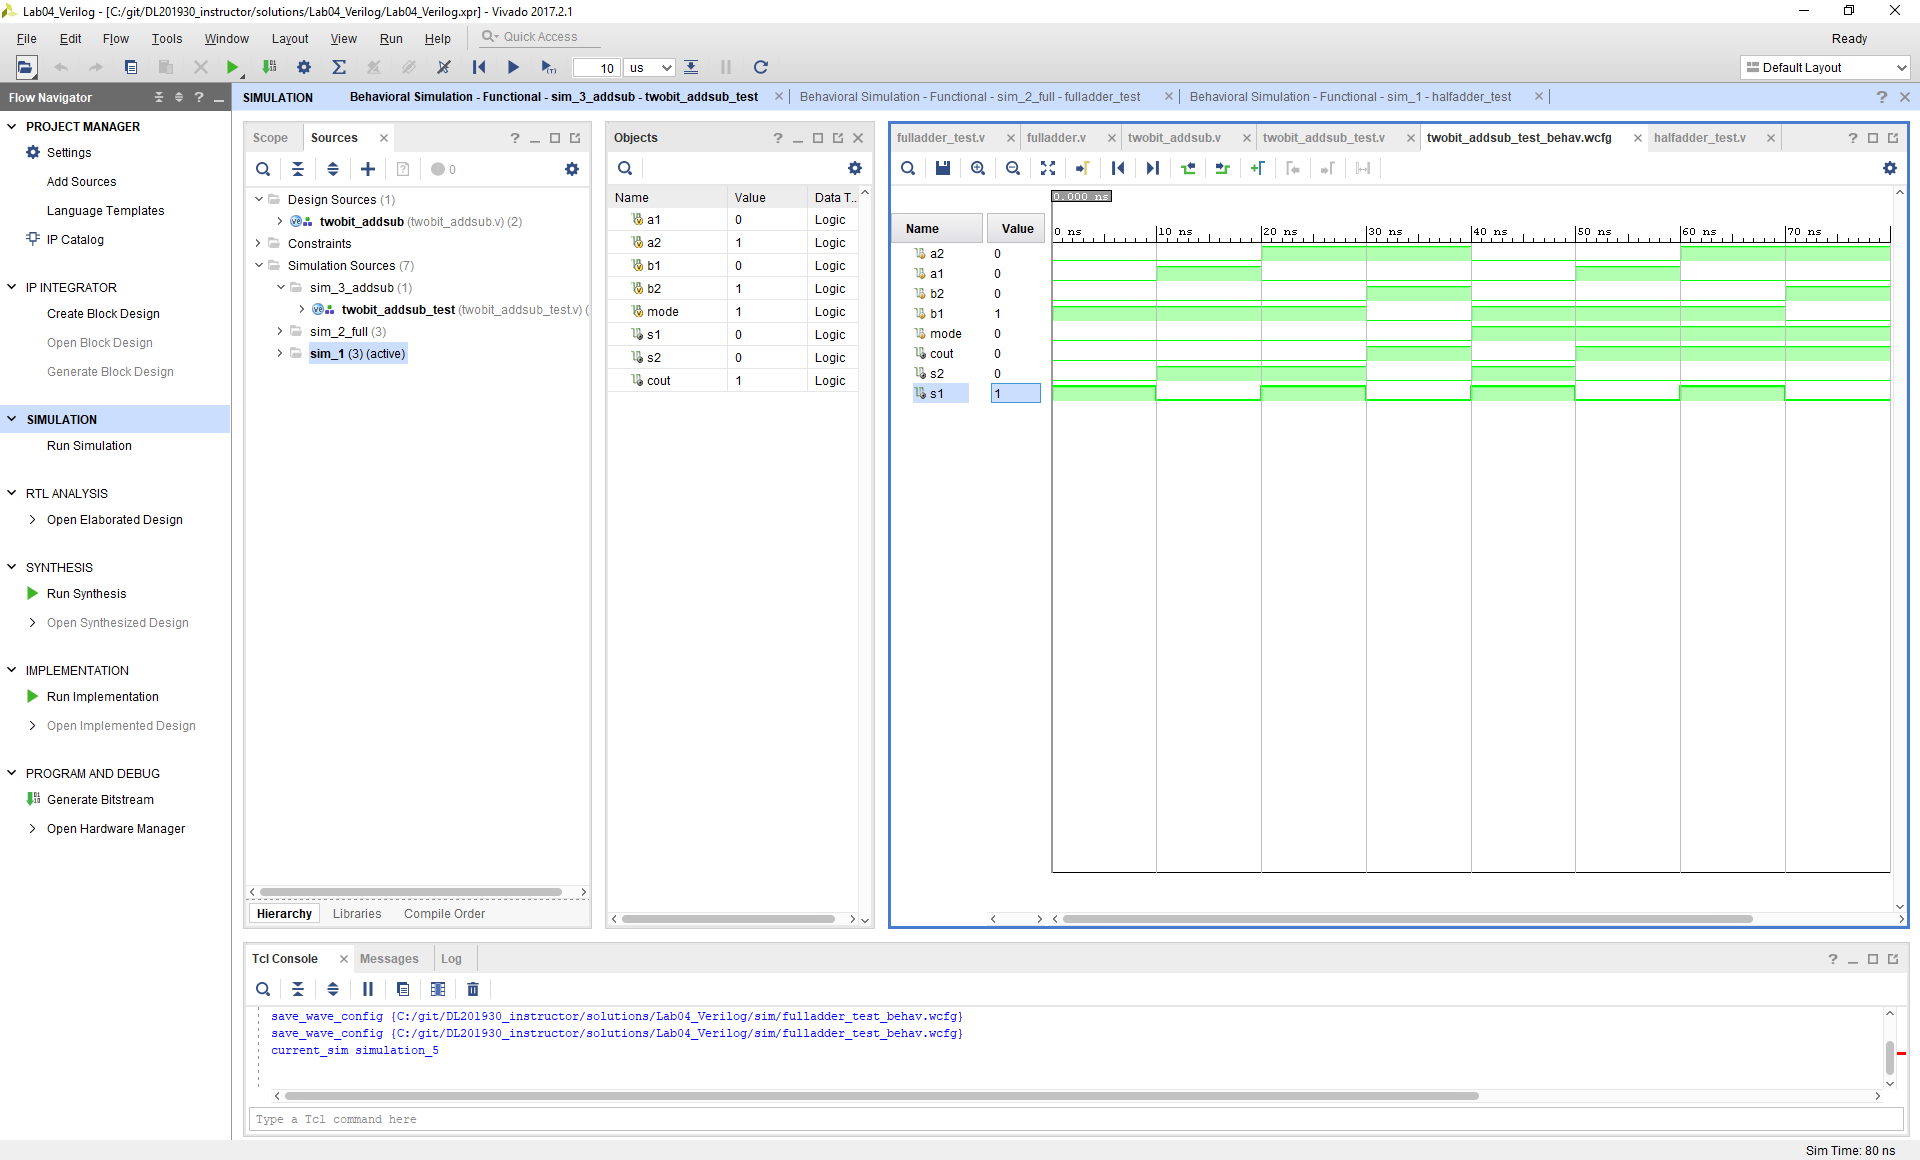
\includegraphics[width=01\textwidth,trim=19cm 15.5cm 0.6cm 4cm,clip]{lab1_example_screenshot}

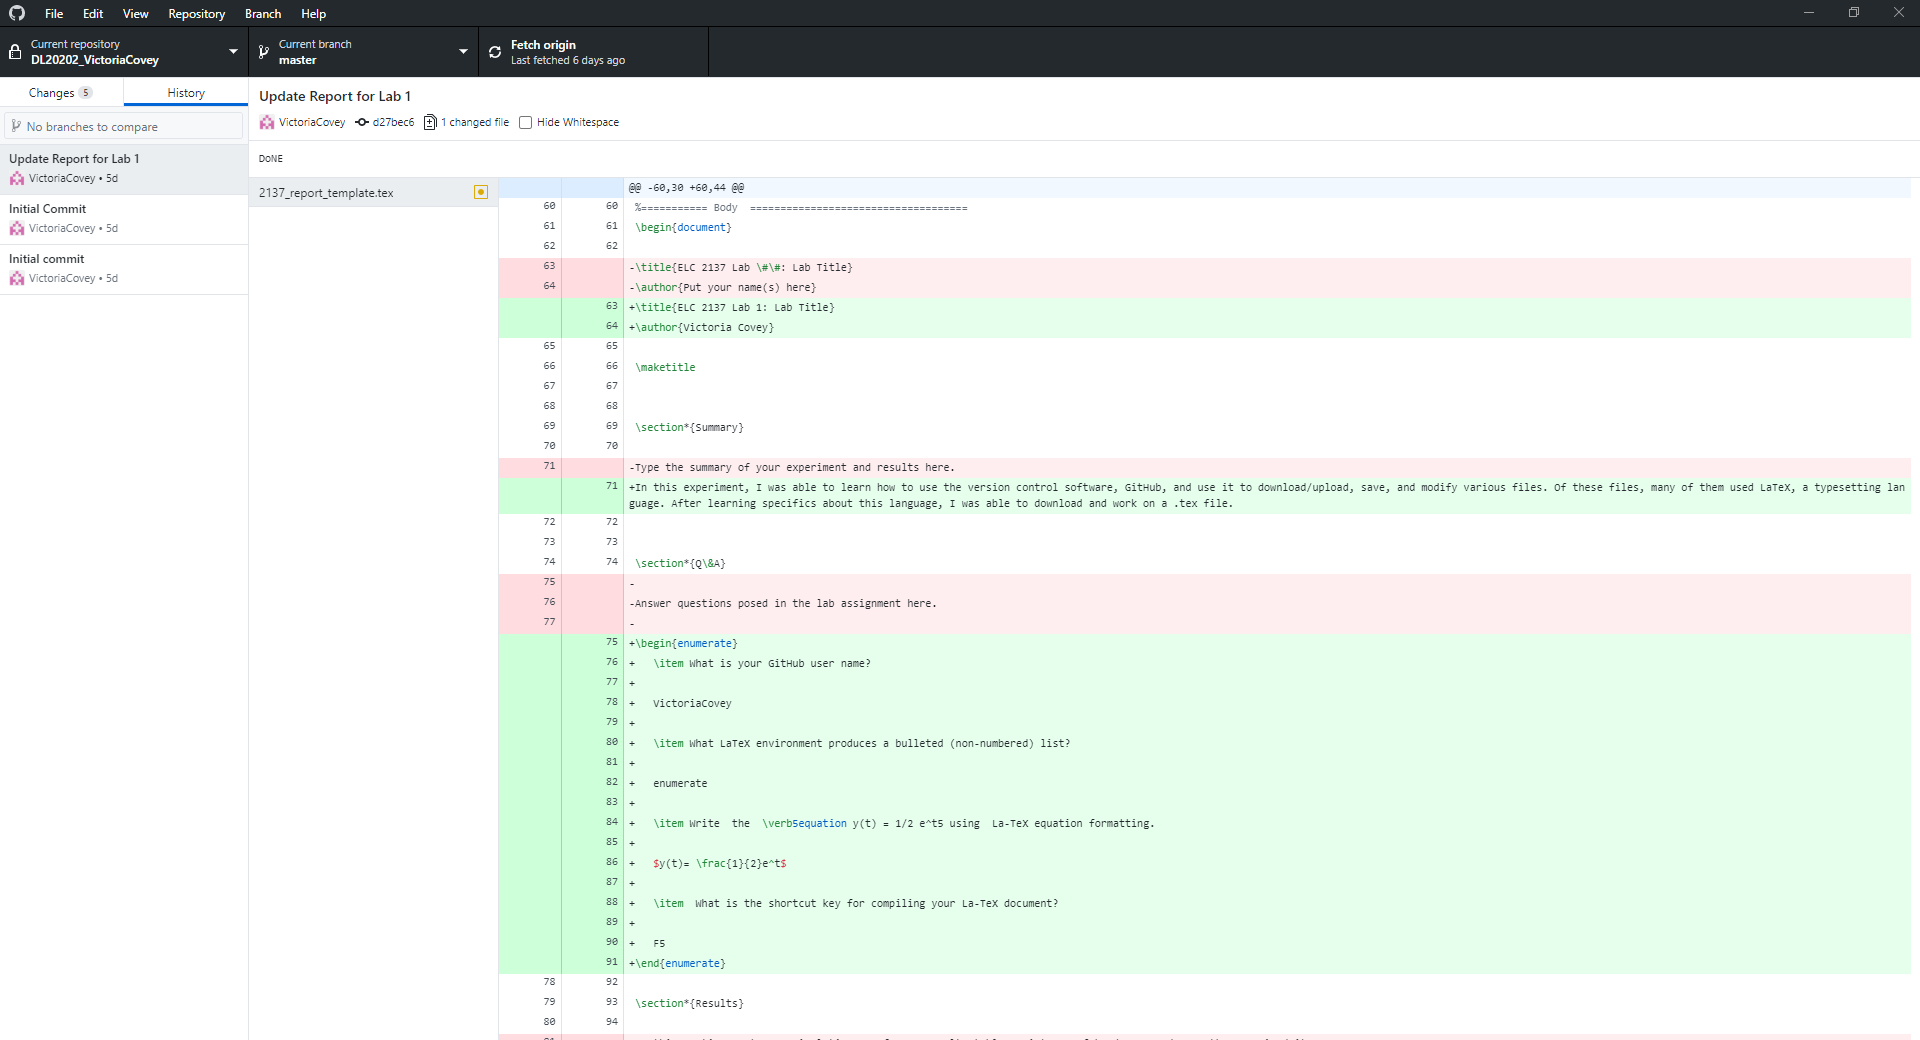
\includegraphics[width=01\textwidth,trim=0cm 6cm 15cm 0.8cm,clip]{GitHub_Screenshot}


\section*{Code}

\Verilog[caption=File-included example code,label=code:file_ex]{lab1_example_code.sv}


\end{document}
